\section{单纯形法与内点法的比较}
\label{sec:lpipm-comparison}

现在两种算法都有了。于是要问：面对一个具体的线性规划，两者各需要做什么、各能交出什么？我们先在同一个工厂问题上把它们并排算一遍，再按稀疏性、内存、退化和再求解几个方面对比。

\paragraph{同一个问题上的两种计算}
工厂问题的标准型是第~\ref{chap:simplex-method}章的数据，$m=3$，$n=5$，最优解是$(4,2,0,0,1)^\top$，最优利润$26$，对偶最优解$\bm{y}^\star=(-2,-1,0)^\top$。单纯形法从基$(3,4,5)$出发，经过$(0,3)$、$(2,3)$，$3$次换基到达最优顶点，每次换基求解一个$3\times3$的基矩阵方程组。

内点法取严格可行起点
\[
 \bm{x}^{(0)}=(1,1,5,7,2)^\top,\qquad\bm{y}^{(0)}=(-3,-3,-3)^\top,\qquad\bm{s}^{(0)}=(5,7,3,3,3)^\top,
\]
这里$\bm{s}^{(0)}=\bm{c}-\bm{A}^\top\bm{y}^{(0)}$，$\mu^{(0)}=10.8$。第一轮的正规矩阵是
\[
 \bm{M}=\bm{A}\bm{D}\bm{A}^\top\approx
 \begin{bmatrix}2.4381&0.6857&0.2857\\0.6857&3.2762&0.1429\\0.2857&0.1429&0.8095\end{bmatrix}.
\]

两种算法都在解$3\times3$的对称或非对称方程组，表面上规模一样，含义却不同。基矩阵只用$\bm{A}$的$3$列，换基时只变一列；$\bm{M}$用到全部$5$列，每轮的数值都变，但元素的稀疏结构不变。

用预测—校正（$\eta=0.99$），$6$轮后互补量从$54$降到约$1.2\times10^{-7}$，点在$4$位小数上就是$(4,2,0,0,1)^\top$。

图~\ref{fig:lpipm-factory-run}把这两个过程画在一起。单纯形法的每一步都站在顶点上，利润单调上升，$3$步后得到精确解。内点法的头几轮就穿过内部接近最优点，第$3$轮已到$25.95$，但此后每轮只是把小数位往后推，点始终不是顶点。

\begin{BookInlineFigure}
  \centering
  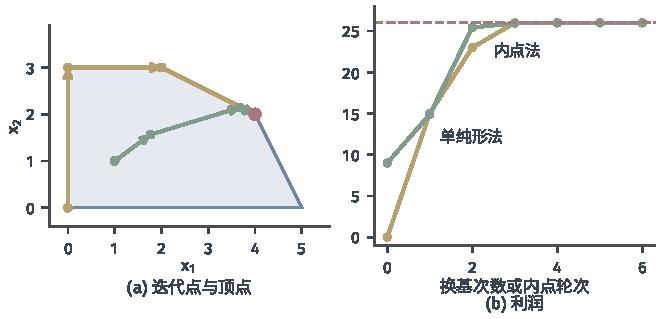
\includegraphics[width=112mm]{figures/05-optimization/01-linear-programming/matplotlib/lpipm-factory-run/figure.pdf}
  \caption{工厂问题上的两种算法。(a)可行域上，黄色是单纯形法的顶点序列，绿色是内点法的前几个迭代点，红点是最优顶点$(4,2)$。(b)利润随迭代的变化，黄线是单纯形法的换基次数，绿线是内点法的轮次，红色虚线是最优值$26$。单纯形法的横轴单位是一次换基，内点法的单位是一次分解$\bm{M}$，两者的代价不同，不能只比轮次。}
  \label{fig:lpipm-factory-run}
\end{BookInlineFigure}

\paragraph{稀疏存储与分解填充}
大规模线性规划的矩阵$\bm{A}$几乎都是稀疏的，这时代价取决于分解时产生多少新的非零元（填充）。两种算法的填充模式不同。

单纯形法分解基矩阵，用LU分解并在换基时更新，只涉及$m$列。内点法分解$\bm{A}\bm{D}\bm{A}^\top$，它的第$(i,k)$个元素非零，当且仅当存在一列在第$i$行和第$k$行都非零。于是只要$\bm{A}$有一列稠密，$\bm{M}$就整个稠密。

图~\ref{fig:lpipm-sparsity}是一个例子：$\bm{A}$是$40\times80$的稀疏矩阵，每列只有两个非零元，再加上一个稠密列。整个$\bm{A}$只有$198$个非零元，$\bm{M}$却有全部$1600$个；去掉那一列后，$\bm{M}$只有$196$个非零元。实现中会把稠密列单独分离出来，用矩阵求逆引理处理，但这需要额外的数值稳定措施。

\begin{BookInlineFigure}
  \centering
  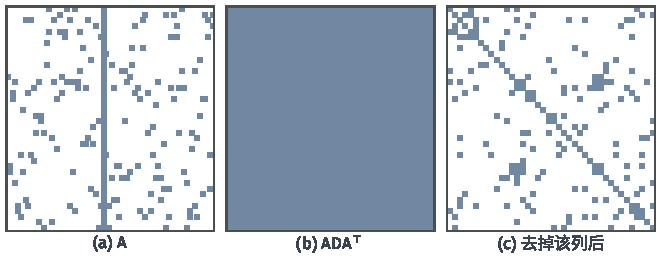
\includegraphics[width=112mm]{figures/05-optimization/01-linear-programming/matplotlib/lpipm-sparsity/figure.pdf}
  \caption{一个稠密列的影响，蓝色方块表示非零元。(a)$40\times80$的稀疏矩阵$\bm{A}$，其中一列稠密。(b)正规矩阵$\bm{A}\bm{D}\bm{A}^\top$完全稠密。(c)去掉该列后的$\bm{A}\bm{D}\bm{A}^\top$仍然稀疏。}
  \label{fig:lpipm-sparsity}
\end{BookInlineFigure}

\paragraph{内存}
内点法每轮要存$\bm{M}$的Cholesky因子，内存由填充决定，并且在整个求解期间都要占用这么多。单纯形法只存基的LU因子，通常比前者小，但可能需要很多次换基。所以问题规模增大时，内点法更容易受内存限制，单纯形法更容易受迭代次数限制，具体哪个先成为瓶颈取决于矩阵结构。

\paragraph{退化与数值性质}
第~\ref{chap:simplex-method}章说明，退化时单纯形法可能原地换基，需要反循环规则。内点法从不访问顶点，路径本身不受退化的基影响，第$t$轮的$\bm{D}$只和当前点有关，因此没有“卡在同一顶点”的现象。

内点法的麻烦在别处。$\bm{D}$的对角元是$x_i/s_i$，随迭代趋于两个极端：最优解中为正的变量对应的元素趋于$+\infty$，为零的变量对应的元素趋于$0$。图~\ref{fig:lpipm-scaling-spread}(a)显示，工厂问题最后几轮对角元的比值已超过$10^{20}$。

\begin{BookInlineFigure}
  \centering
  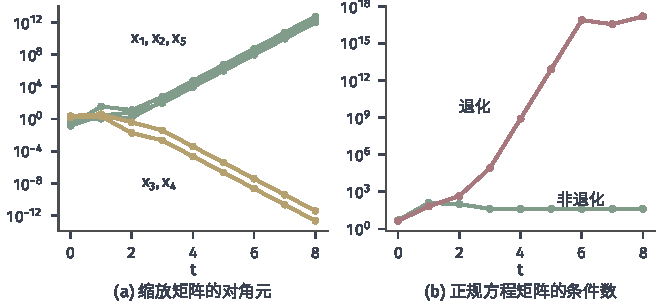
\includegraphics[width=112mm]{figures/05-optimization/01-linear-programming/matplotlib/lpipm-scaling-spread/figure.pdf}
  \caption{缩放矩阵与条件数的变化，预测—校正，$\eta=0.99$。(a)工厂问题中$D_{ii}=x_i/s_i$随轮次的变化，绿线对应最优解中为正的$x_1,x_2,x_5$，黄线对应为零的$x_3,x_4$。(b)$\bm{M}=\bm{A}\bm{D}\bm{A}^\top$的$2$范数条件数：绿线是非退化的工厂问题，红线是再加一条约束$x_1+x_2\leq6$使最优顶点退化的情形。}
  \label{fig:lpipm-scaling-spread}
\end{BookInlineFigure}

这种悬殊看起来很危险，影响却取决于问题的结构。图~\ref{fig:lpipm-scaling-spread}(b)的绿线说明，非退化时$\bm{M}$由三个正的基变量主导，它们的$D_{ii}$同步增大，条件数稳定在约$41$。红线是最优顶点退化的情形，正变量少于$m$个，$\bm{M}$趋于奇异，条件数涨到$10^{16}$以上。

大的条件数并不直接意味着算出的方向没用：误差往往落在对后续更新影响不大的子空间里，这是内点法在实践中比条件数预示的更稳健的原因，但这需要专门的误差分析，读者可查阅专著\scite{math-nocedal2006numerical}。求解器还要辅以正则化和迭代精化。最终都应当检查残差，不能只凭条件数判断。

\paragraph{基与再求解}
单纯形法返回一个基，这使很多后续工作很方便：约束或目标有微小改变时，从原来的基接着做，往往几次换基就够（第~\ref{chap:simplex-method}章的对偶单纯形法）；固定基的参数分析可以直接读出结论成立的范围。

内点法也返回对偶信息，这些$\bm{y}$和$\bm{s}$的值可以当作影子价格用，但结果是最优面中央的一个点，解不唯一时它和某个基给出的对偶解并不相同。需要基时要做上一节的基恢复。

内点法的热启动也比较困难。上一次的解贴近边界，某些$x_i$或$s_i$接近零，从这里出发的步长通常很短，反而不如重新开始。因此在分支限界这类需要大量相关求解的场景中，单纯形法更占优势，这也是两种方法长期并存的原因之一。

\paragraph{速度取决于问题和实现}
两种算法都不总是更快。一般而言，内点法在规模很大且$\bm{M}$稀疏时往往轮数少、速度快，单纯形法在$\bm{M}$稠密或需要反复热启动时更有优势。这只是经验性的倾向，具体结果要看矩阵结构、预处理和实现水平，求解器通常提供两者甚至并行运行。

表~\ref{tab:lpipm-compare}总结了本节的对比。

\begin{table*}[!htbp]
  \centering
  \begin{tabular}{@{}lll@{}}
    \toprule
    方面 & 单纯形法 & 内点法\\
    \midrule
    每步的工作 & 解基矩阵方程，换一列 & 分解$\bm{A}\bm{D}\bm{A}^\top$，全部列参与\\
    迭代次数 & 随结构变化，最坏情形指数 & 通常很少，短步规则有$O(\sqrt{n}\log(1/\varepsilon))$的界\\
    稀疏结构 & 基的LU因子，变化较小 & 稠密列会使$\bm{M}$稠密，需特殊处理\\
    内存 & 通常较小 & 由Cholesky填充决定，通常较大\\
    退化 & 可能原地换基，需反循环规则 & 不停滞，但$\bm{M}$可能病态\\
    交出的结果 & 基、顶点解、对偶解 & 内部的近似点和对偶量，需要基时另作恢复\\
    再求解 & 从旧基热启动较容易 & 从旧解热启动较困难\\
    \bottomrule
  \end{tabular}
  \caption{单纯形法与内点法的对比。各项是对典型情形的概括，速度结论取决于问题结构和实现。无论用哪种方法，浮点实现都要检验可行性和最优性。}
  \label{tab:lpipm-compare}
\end{table*}
